\chapter{Simulator}

We will go through a few arguments to underline that this is a good investment for time saving of future development.


\subparagraph{Debugging / Design Test}
Everybody that has already run FPGA designs in hardware knows that it is really hard to properly debug them in case of errors happening (e.g. deadlocks, etc.), since there is no notion of setting a breakpoint and look at the intermediate values as we are used to do this in software. What you can do is setting up a debug channel, which enables you to see at least what is happening on the device or where it breaks, but the capabilities remain very limited. \\
That's why we want the functionality to simulate the design in software first in order to eliminate as many bugs as possible. In case of problems, we can detect and debug them in the integrated development environment which gives us access to the current state of the whole design. This significantly reduces the error rate and increases the certainty of running on the actual hardware without issues.


\subparagraph{Correctness}
Furthermore, changes in the code generator, which will often occur in the future while doing the low-level performance optimization, might result in a working design, that produces invalid output data. Running the same input data on the simulator and compare the computation result to the one from the hardware gives us the opportunity to check the correctness of the hardware design without having to write a  dedicated golden model implementation for every problem.


\subparagraph{Performance Metrics}
Running the design in software gives us the benefit of being able to collect whatsoever information or metric we are interested in. This means that we cannot only test the design for correctness, but we can for example find out if the buffer size estimate is tight, in other words, that is the size exact and not just large enough.


\section{FPGA Execution Model}
The software execution model of the abstracted FPGA device is modular built up and transitions multiple phases, which we will have a look at now.


\subsection{Initialization}
In the initialization phase, we set up and load all input data into their corresponding allocated location. This is similar to the transfer of the input data from the host memory to the reconfigurable device.


\subsection{Step Execution}
After initialization we can start with the actual execution process. A single run of the so called step execution represents a clock cycle on the actual hardware. This is repeated till the stop condition is met, which will end the execution and initiates the transition over to the finalization process.  
\begin{figure}[h]
	\centering
	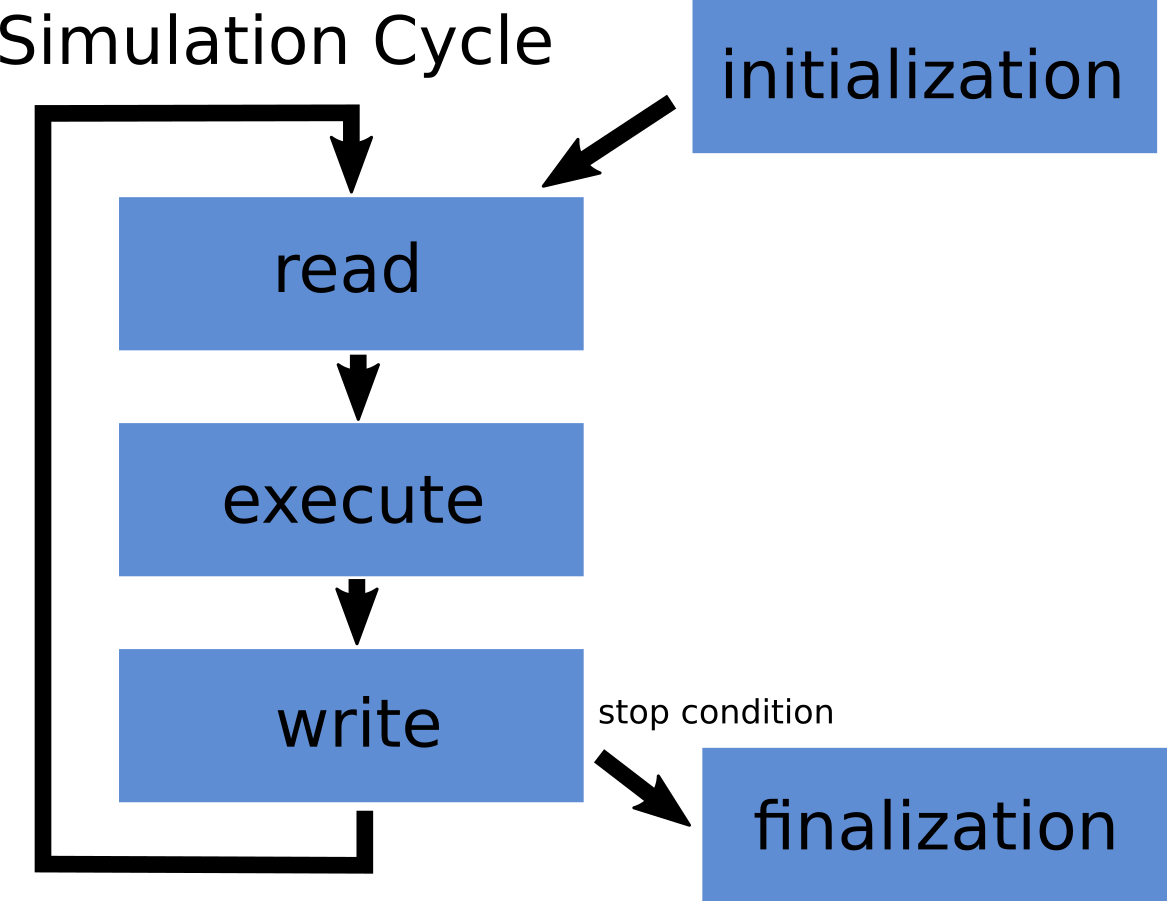
\includegraphics[height=12em]{drawings/simulator-simulation-cycle.png}
	\caption{Simulation Cycle: Step by step execution.}
	\label{fig:simulator-simulation-cycle}
\end{figure}


\subparagraph{Read}
In the read phase, all kernels check if data is available from all input channels. If this is the case they can consume them.


\subparagraph{Execute}
In the execution phase, all kernels that have successfully read data elements from all input channels can compute the output value according to the kernel function. In order to account for the operation latencies, the result is not directly written to the output channel, but rather hold back for \textit{latency} cycles.


\subparagraph{Write}
In the write phase, all kernels with valid output data write the result to the output channels, which are either input channels of other kernels or the channel collecting the final result for the transfer back to the host memory.


\subparagraph{Stop Condition}
The problem size respectively the number of data elements to process is given in the problem definition. Therefore we know after every kernel has written that many elements to the output channels, we can safely switch to the finalization phase.


\subparagraph{Finalization}
The finalization process takes care of writing the final result to the filing system.


\section{Performance Metrics}


\subparagraph{Buffer Utilization}
We are not only interested in the information of having large enough buffers, but also for example if they are actually filled 100\% at some instance in time. If this would not be the case we could reduce their size and therefore save buffer space. Furthermore, we might, at some point, come up with a stencil program or kernel merging strategy that might reduce the peak buffer size usage and therefore could reduce the overall memory consumption.


\subparagraph{Start and End Time}
Another interesting per-kernel metric is the timing of the actual start (program counter time) and end time. This allows us to see if there are any stalls happening for this kernel.



\section{Error Handling}
The buffer optimization goal is to make all buffers (internal and delay buffers) as large as necessary, but as small as possible. In case of a kernel producing a valid output data element, but any of the output channels is already full indicates that the buffer was too small. This holds true since we are running the design synchronously. In such a case, we can output the current state of the simulation (buffer data, performance metrics, etc) which gives us the possibility to resolve these issues in software.


\section{Conclusion}
The software simulation gives us great flexibility and insight into understanding what is happening on the hardware itself and helps us to prevent and detect bugs in an early stage where we still have the freedom to see into the global simulator state. Furthermore, we can gain great insights into performance measures which might lead to optimization and better use of the hardware resources.
